\chapter{A New Recruit}

% Une partie destinée à un nouvel arrivant dans la société qui va reprendre / poursuivre le projet dans lequel vous avez été impliqué. Il faut donc lui décrire le contexte de l’entreprise, du projet, l’architecture générale de celui-ci, le contexte et l’organisation de l’équipe de travail, le tout de façon synthétique. Il faudra également y apporter les précisions quant aux difficultés rencontrées dans le projet.

This part has for objective to onboard a new recruit in a project that I worked on during my internship which is \gls{san-iscsi-csi}, developped as an \glsdef{open-source} software on \glsdef{github}. This software allows to perform \glsdef{dynamic-volume-provisioning} on \glsdef{k8s} and \glsdefs{csi}-compliant \glsdeff{\glspl}{k8s-co}.

\clearpage

\section{Introduction}

In order to onboard you on our project \gls{san-iscsi-csi}, we will review some information you should know about it and about the company \gls{enix} more generally.

We will first discuss the company context, followed by the project context and its general architecture and finally describe the context and organisation of the project work team.

\section{Company context}

\gls{enix} SAS is a company selling \glsdef{cloud}, \glsdef{devops} and \glsdef{k8s} services in a \glsdefs{b2b} business model. The company has been created in the early 2000s in the LAN parties environment. Sébastien, Romain, Alexandre, Jérôme and Laurent, student then, started this company in response to needs in infrastructure and networking during those events.

Today, \gls{enix} counts 15 employees and a few external collaborators. We work for some big clients like \gls{xbto}, \gls{tdf}, \gls{maif}, \gls{ulule}, \gls{airbus} and others.

\section{Project context}

The idea from which \gls{san-iscsi-csi} came from is the one to implement all cutting-edge features of \glsdef{k8s} in terms of storage, using storage appliances initially not intended for this purpose. It targets mainly \glsdef{on-prem} \glsdef{cloud} infrastructures.

\subsection{Cloud context}

Nowadays, \glsdef{containerization} (see \figref{fig:containers}) of applications has become a golden standard in the industry. It allows to build, ship and run applications anywhere \glsdef{on-prem} or in the \glsdef{cloud}, with particular focus on portability and operability. \glsdeff{\glspl}{container} allow to run softwares in a sandboxed environment, which increase security and are lighter than \glsdeff{\glspl}{virtual-machine} which require a full \glsdefs{os} running for each instances.

\begin{figure}[h]
    \centering
    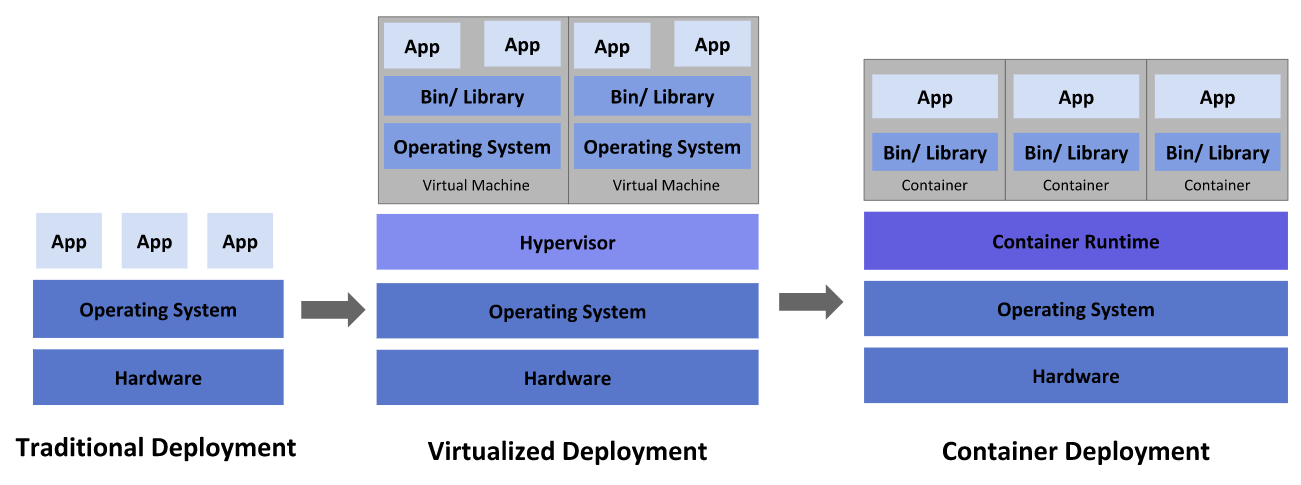
\includegraphics[width=\textwidth]{schema-containers.png}
    \caption{From traditional to containerized deployments}
    \label{fig:containers}
\end{figure}

A solution like \glsdef{k8s} is used to orchestrate \glsdeff{\glspl}{container} and is able to manage the whole underlying infrastructure (network, storage, databases, etc...). It is composed of several specialized services that operate a set of \glsdeff{\glspl}{container} in the right conditions.

As shown in \figref{fig:k8s-components}, there is on one hand the control plane, which control the state of the \glsdef{cluster}, and on the other hand \glsdef{k8s} \glsdeff{\glspl}{k8s-node}, which are servers running orchestrated \glsdeff{\glspl}{container}.

\begin{figure}[h]
    \centering
    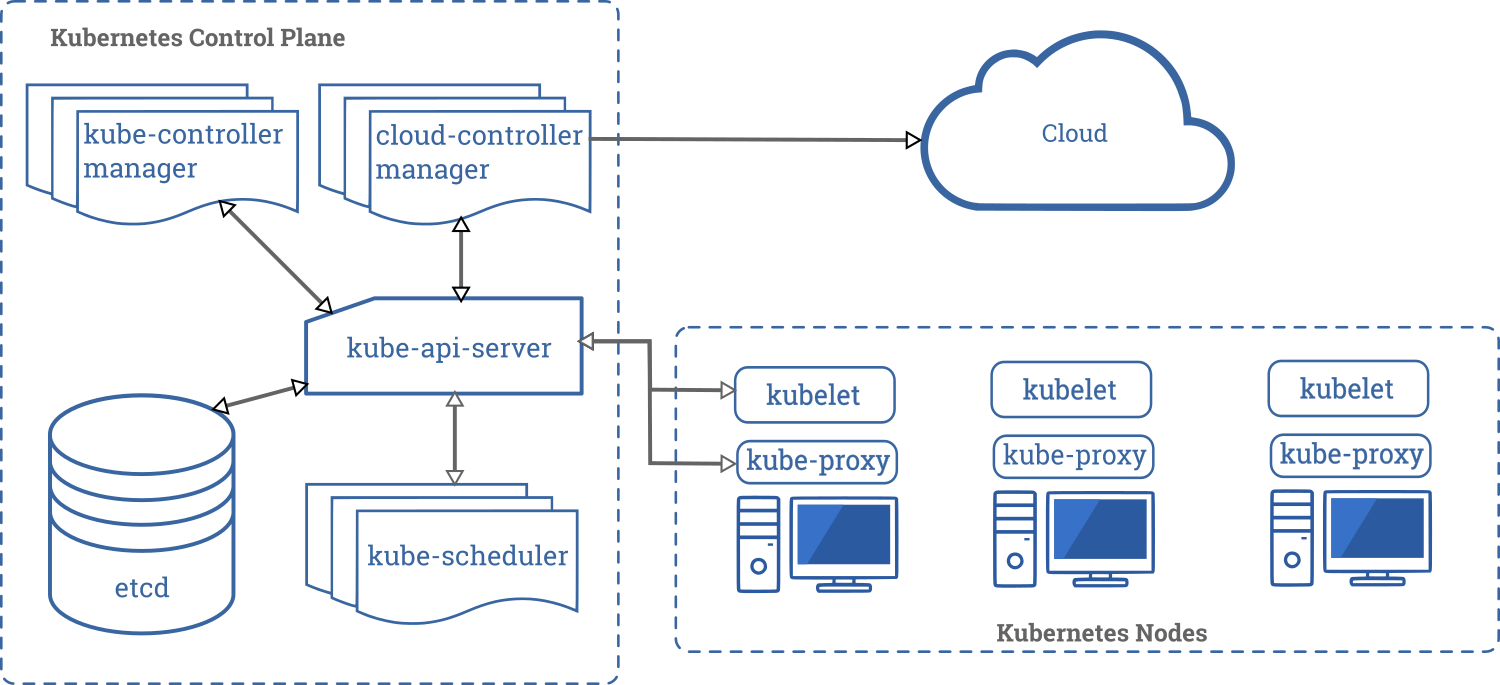
\includegraphics[width=\textwidth]{schema-kubernetes-components.png}
    \caption{Kubernetes components}
    \label{fig:k8s-components}
\end{figure}

On the storage side comes the concept of \glsdef{volume}, which is actually a storage unit. A volume can be persistant or not, local or distant, dynamically or statically provisioned. Statically means that the \glsdef{volume} has been provisioned by someone manually, whereas dynamically means that someone only asked to have a \glsdef{volume} available and some software got the work done.

\glsdef{csi} is a standard that comes to unify the process of \glsdef{dynamic-volume-provisioning} across \glsdeff{\glspl}{k8s-co}. It allows to dynamically provisioning of \glsdef{k8s-pv} through a configuration object called \glsdef{k8s-pvc}.

\subsection{Typical storage solution}

Dot Hill Systems Corp, bought by Seagate in 2015, build since 1997 inexpensive storage appliances. Models available since years now have typical expected features and are rebranded by several constructors such as Dell or HP and so on. We choosed to implement our \glsdef{csi} plugin and make it compatible with a group of appliances provided by seagate.

The feature that comes handy in the context of \gls{san-iscsi-csi} is the availability of a well documented \glsdefs{api}, almost fully cross-compatible between models, versionned and allowing to control them remotely.

\subsection{Technical opportinity}

\glsdef{k8s} allows to manage \glsdeff{\glspl}{container} persistant storage thanks to \glsdef{k8s-pv}. The state of the art strategy is to provide \glsdeff{\glspl}{volume} on the fly, also called \glsdef{dynamic-volume-provisioning}.

The list of supported \glsdeff{\glspl}{volume} is consequent, see \href{https://kubernetes.io/docs/concepts/storage/volumes/\#types-of-volumes}{Kubernetes - Types of Volumes}. Some \glsdeff{\glspl}{volume} make use of the \glsdef{iscsi} protocol, which is the one used by Seagate appliances as well, but this protocol don't natively support \glsdef{dynamic-volume-provisioning}. It is that precise need that \gls{san-iscsi-csi} tries to fulfill.

\section{General project architecture}

\subsection{Working principle}

\glsdef{k8s} \glsdefs{api} expose two resources which are storage requests (\glsdef{k8s-pvc}) and storage units (\glsdef{k8s-pv}). Applications can create \glsdeff{\glspl}{k8s-pvc} and the \glsdef{k8s} control plane will try to satisfy those requests through our \glsdef{csi} plugin, creating \glsdeff{\glspl}{k8s-pv} for the applications.

\subsection{CSI specification}

\glsdef{csi} specification connects two components: a \glsdef{k8s-co} and a \glsdef{k8s-sp}. The job of a \glsdef{csi} plugin is to do the middleman between them. The advantage of such an architecture is to make possible to develop a plugin once, and use it with every \glsdef{k8s-co} \glsdef{csi}-compatible.

The \glsdef{k8s-co} will be able to ask the \glsdef{k8s-sp} to create a \glsdef{volume} with a specified size, resize it, and eventually delete it. It can ask the \glsdef{k8s-sp} to make storage available on a specific server. It allows to easily change the location of a certain \glsdef{volume}, allowing it to move in coordination with \glsdeff{\glspl}{container} using it across a \glsdef{cluster}.

\subsection{iSCSI protocol}

As said earlier, the appliance we choosed support the portocol \glsdef{iscsi}. \glsdef{iscsi} is a protocol that emulate the SCSI protocol over a network, like internet for instance. SCSI define how to link a computer with a storage device like a hard drive for example.

Thanks to this protocol, we are able to link disks from the storage appliance to servers in a \glsdef{k8s} \glsdef{cluster}.

In order to make the appliance highly availabile, it includes hardware redundancy of its controller, which is the part that allows communication with disks. This way, if one controller dies, there is still one available until the other is repaired or changed. This, however, had introduced some difficulties described later in this document.

\subsection{General overview}

A \glsdef{csi} plugin is composed of two parts, a node, and a controller. The controller will control the appliance in order to make disks of required sizes available, resize them, and so on.., whereas the node will use the \glsdef{iscsi} protocol to link disks to servers where they run.

There will be one controller per \glsdef{cluster}, and one node per \glsdef{k8s} \glsdef{k8s-node}. It can be tricky, but don't get confused between a \glsdef{csi} node (a software part of the plugin) and a \glsdef{k8s} \glsdef{k8s-node}, which is a server. Both node and controller servers receive \glsdef{csi} commands from \glsdef{k8s} through \glsdeff{\acrshort}{grpc}.

\begin{figure}[h]
    \centering
    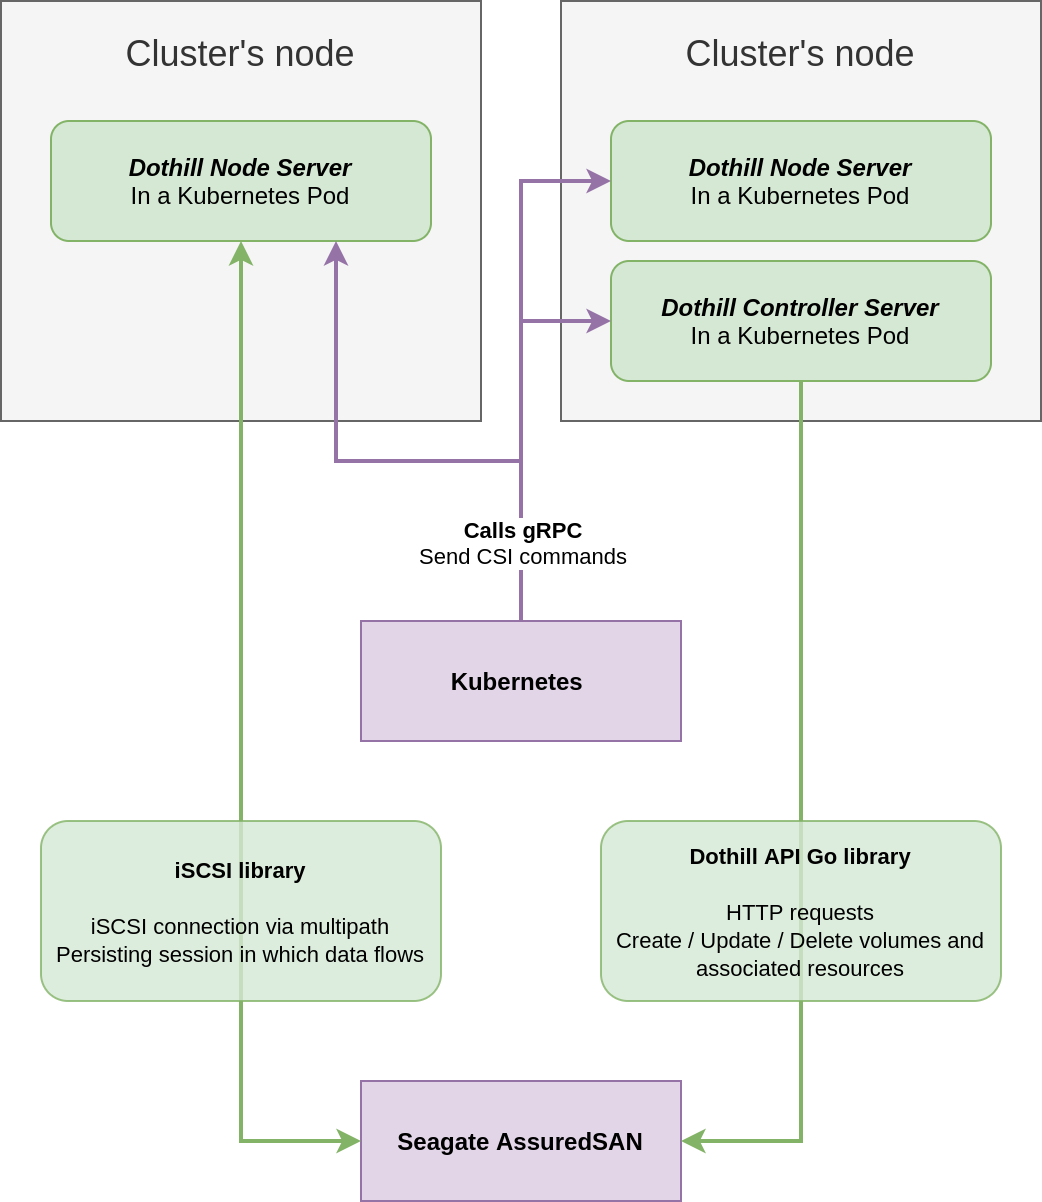
\includegraphics[width=10cm]{schema-san-iscsi-csi-simplified.png}
    \caption{Interactions between \glsdef{k8s} and \gls{san-iscsi-csi}}
    \label{fig:k8s-san-scsi-csi}
\end{figure}

As you can see in the schema above, a last piece of software we didn't describe yet is the Dothill API Go library. It's a \glsdef{library} that we also open-sourced and that allows to control the storage appliance.

\subsection{Difficulties encountered}

In a previous section, we talked about difficulties introduced by the use of \glsdef{iscsi} and the fact that the Seagate appliance supports controllers redundancy. In order to use this feature, several \glsdef{iscsi} connexions have to be opened. But each connexion will be shown on the client computer as an individual disk. And here comes a last tool called \glsdef{multipathd}. This tool allows to take several disks, and show them as one single disk. If one disk fail because the connexion or the controller failed, there is still at least one disk working, so the main disk created by \glsdef{multipathd} will still be working.

\glsdef{multipathd} is an old tool that has been designed in the optic to be used by humans. It means that disks will be plugged and unplugged quite slowly compared to what a computer is capable of. With \gls{san-iscsi-csi}, plugging and unplugging disks is done by the plugin, not directly by a human. We thus started to face some \glsdef{concurrency} issues. For some surprising reasons, it happens that disks on the computer representing different disks on the appliance will be grouped together by \glsdef{multipathd}, which can cause some severe issues on the disk, including \glsdef{fs-corruption}.

We spent several weeks on the issue already and \glsdef{multipathd} still seems to behave erratically. We however discovered many aspects of this tool and progressed in its understanding. But \glsdef{multipathd} is a very complex software and its community isn't that big, meaning that it's hard to find answers to some questions. We still have a lot to do around this subject, but a lot has been done too.

\section{Work team}

\subsection{Context}

\subsection{Organization}

\clearpage
